\section{Phân tích các biến phân loại}
\label{sec:3_6}
Mỗi thuộc tính được thống kê đủ các mức quan sát trên dữ liệu phát triển, với một mức riêng cho giá trị thiếu. Với biến có trên mười mức, biểu đồ gộp phần còn lại để dễ đọc; các bảng CSV vẫn giữ đầy đủ mọi mức.

\begin{table}[htbp]
\centering
\small
\caption{Tóm tắt các thuộc tính phân loại trên adult.data gốc}\label{tab:categorical-summary}
\begin{tabular}{lp{.16\textwidth}p{.28\textwidth}r}
\toprule
Thuộc tính & Số mức kể cả thiếu & Mức phổ biến nhất & Tỷ lệ (\%) \\
\midrule
workclass & 9 & Private & 69,70 \\
education & 16 & HS-grad & 32,25 \\
marital-status & 7 & Married-civ-spouse & 45,99 \\
occupation & 15 & Prof-specialty & 12,71 \\
relationship & 6 & Husband & 40,52 \\
race & 5 & White & 85,43 \\
sex & 2 & Male & 66,92 \\
native-country & 42 & United-States & 89,59 \\
\bottomrule
\end{tabular}
\end{table}

\begin{figure}[htbp]
\centering
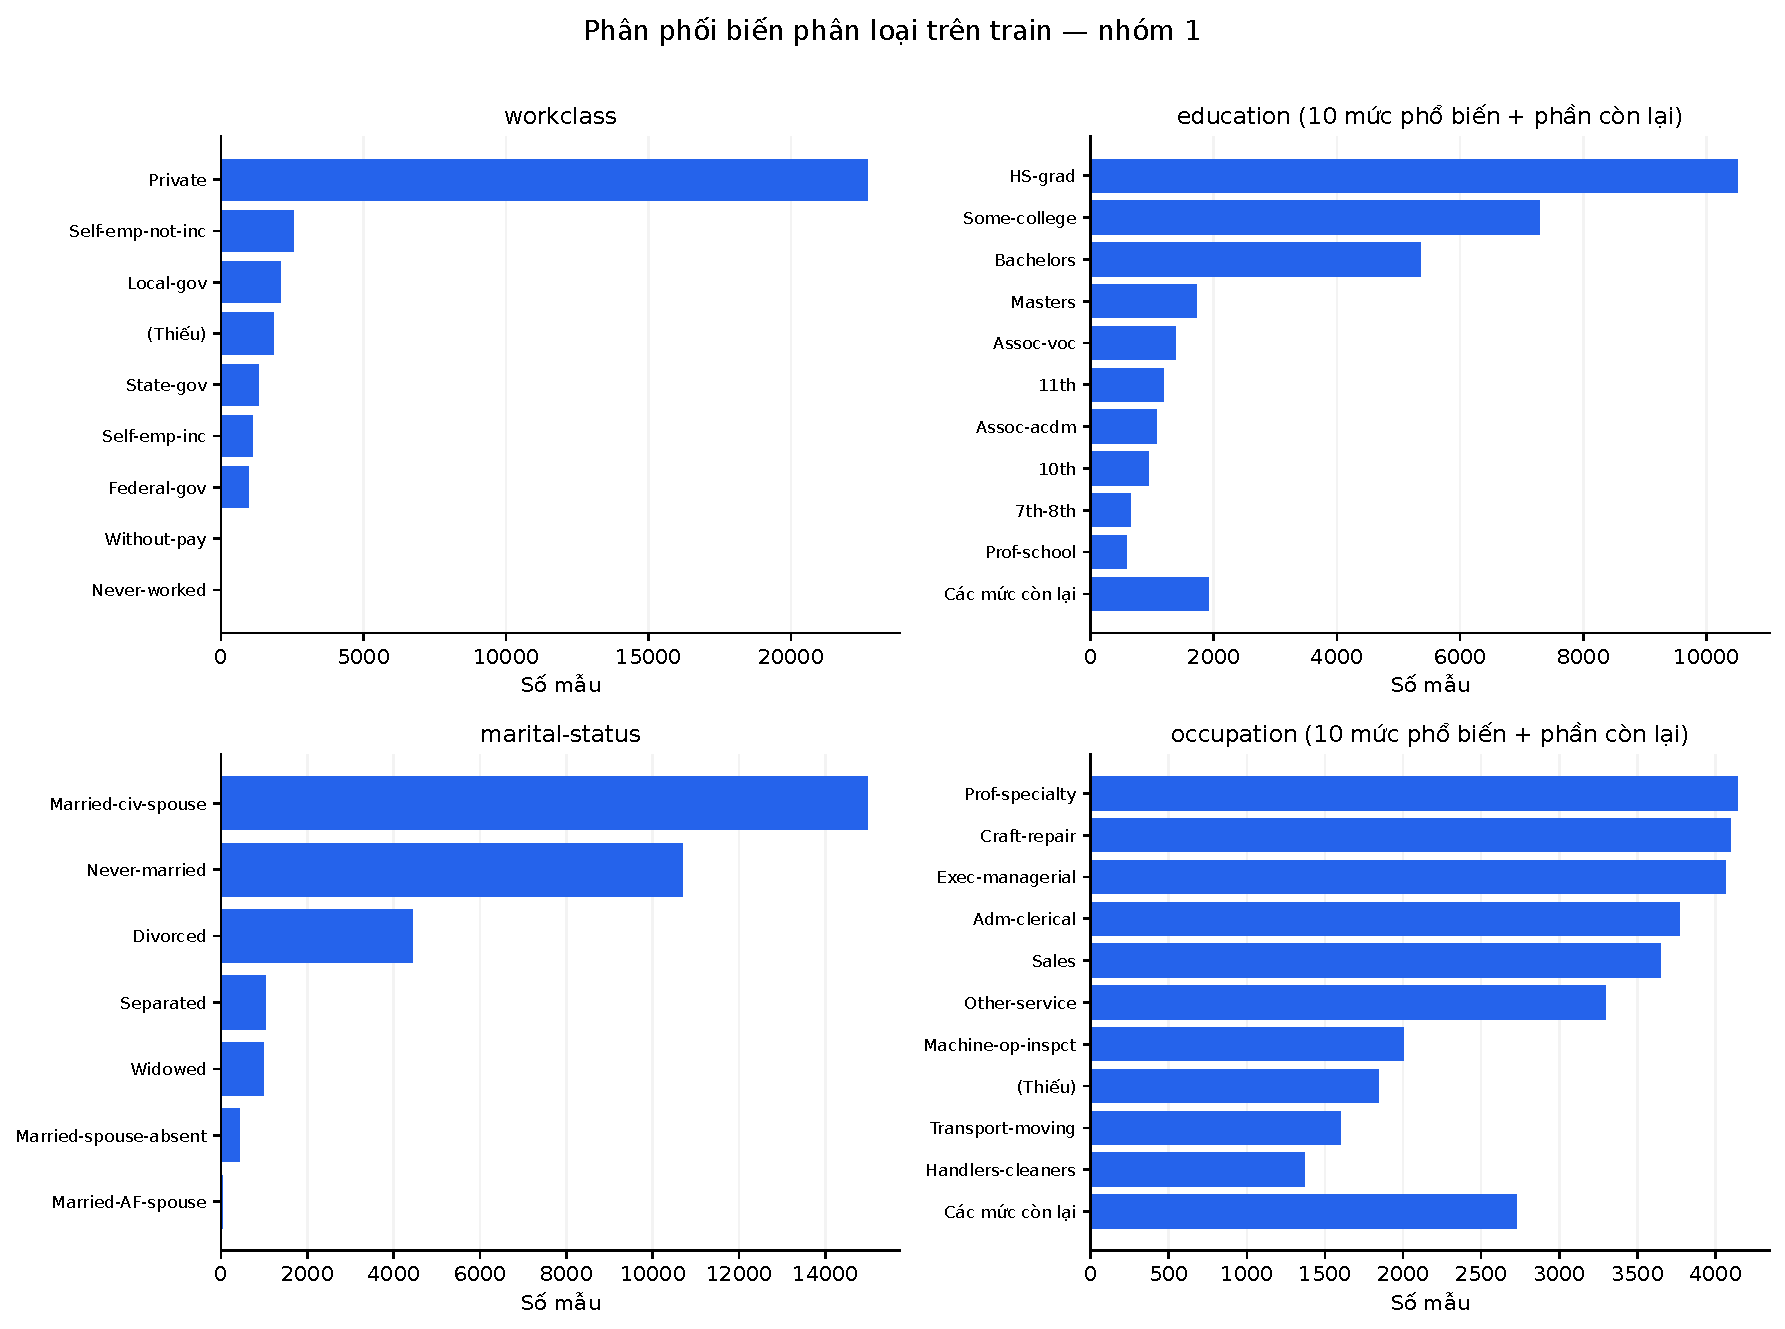
\includegraphics[width=.92\textwidth,height=.72\textheight,keepaspectratio]{Images/chapter_3/3_6/categorical_counts_1.pdf}
\caption{Phân phối workclass, education, marital-status và occupation}
\label{fig:categorical-1}
\end{figure}

\begin{figure}[htbp]
\centering
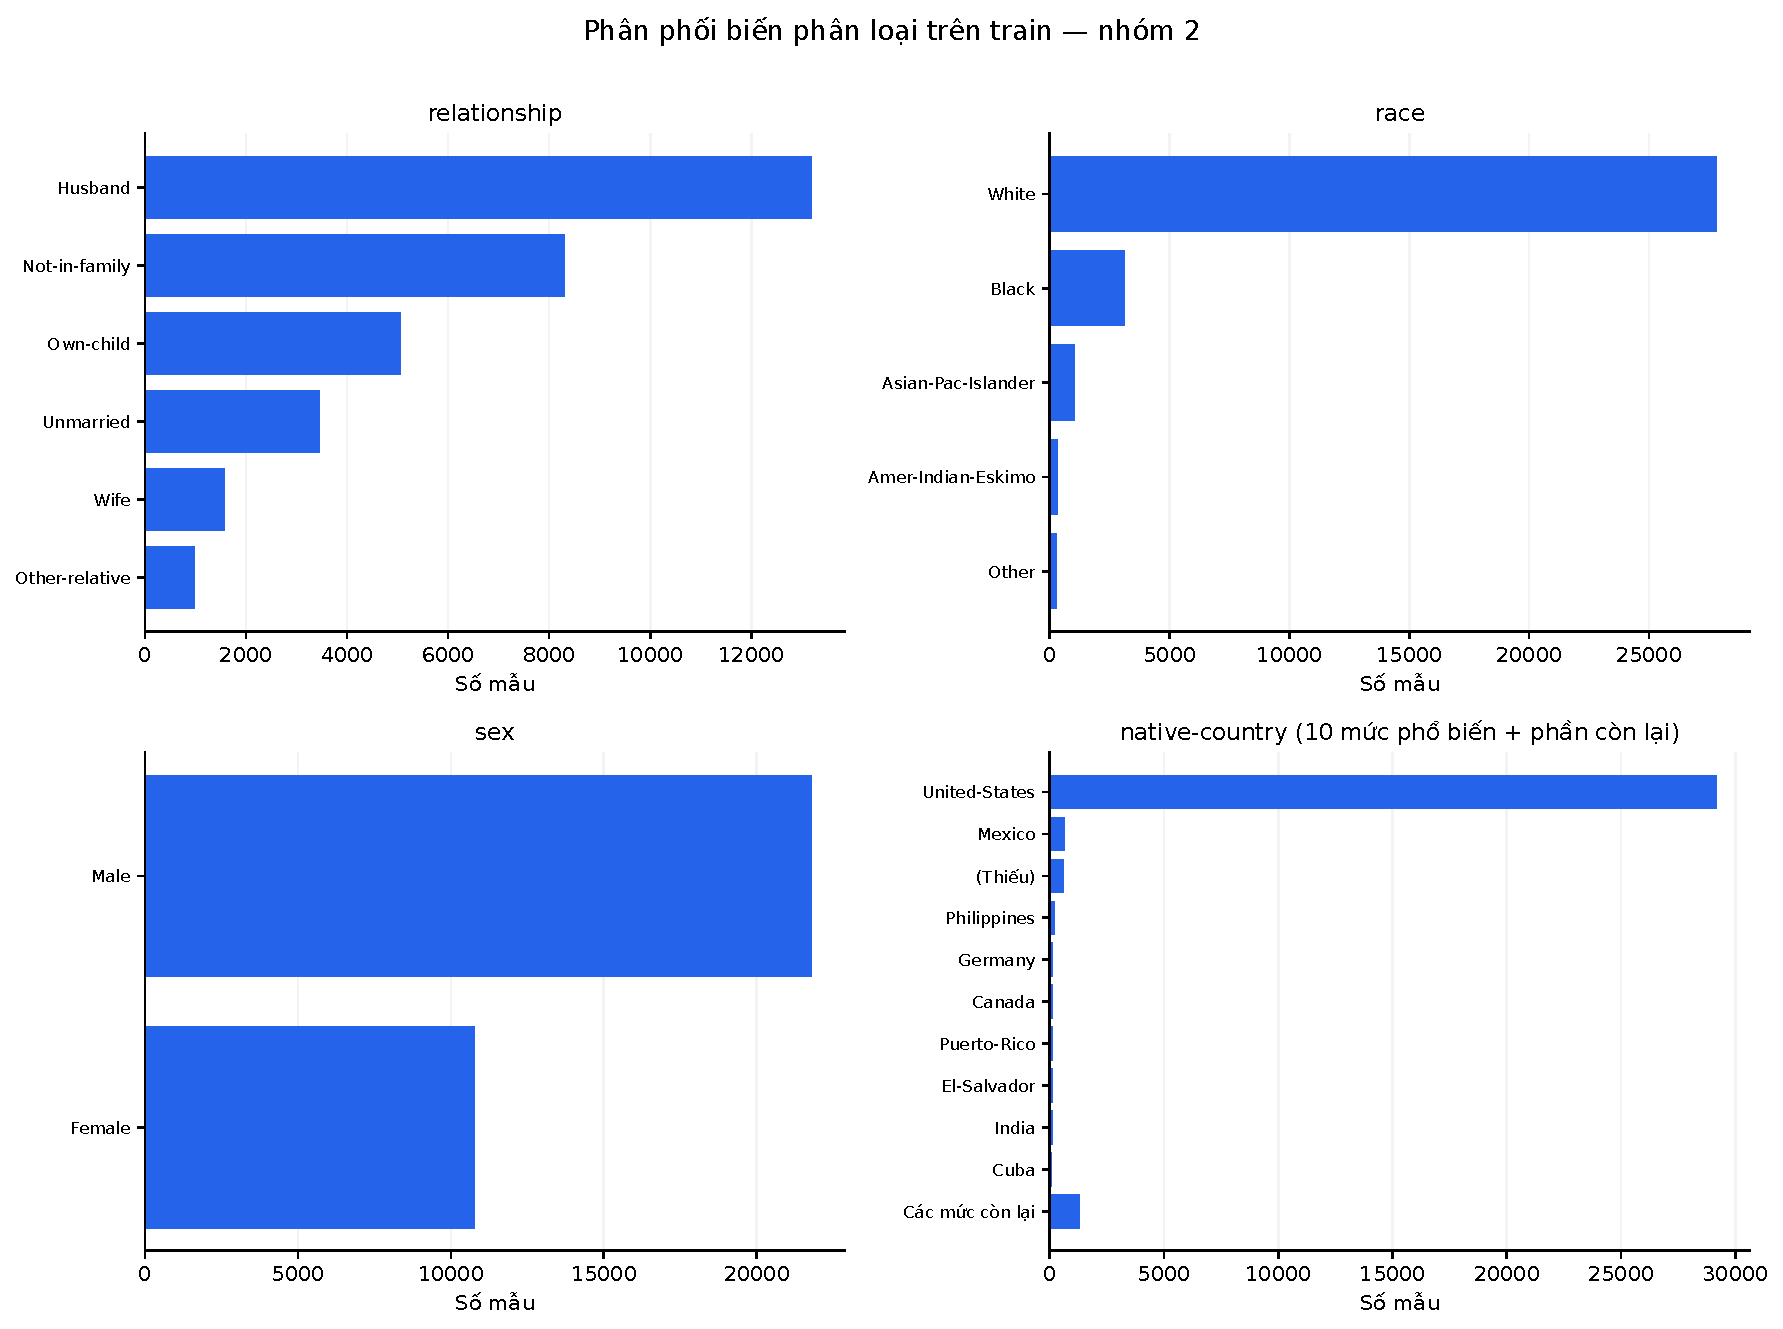
\includegraphics[width=.92\textwidth,height=.72\textheight,keepaspectratio]{Images/chapter_3/3_6/categorical_counts_2.pdf}
\caption{Phân phối relationship, race, sex và native-country}
\label{fig:categorical-2}
\end{figure}

Biểu đồ theo học vấn bổ sung tỷ lệ nhãn \texttt{>50K} trong từng nhóm và số mẫu làm mẫu số. Đây là mối liên hệ mô tả trên dữ liệu quan sát, không được diễn giải thành tác động nhân quả. Khi so sánh tỷ lệ cần chú ý các nhóm có ít mẫu; các tỷ lệ này chưa được dùng để chọn siêu tham số hoặc xếp hạng mô hình.

\begin{figure}[htbp]
\centering
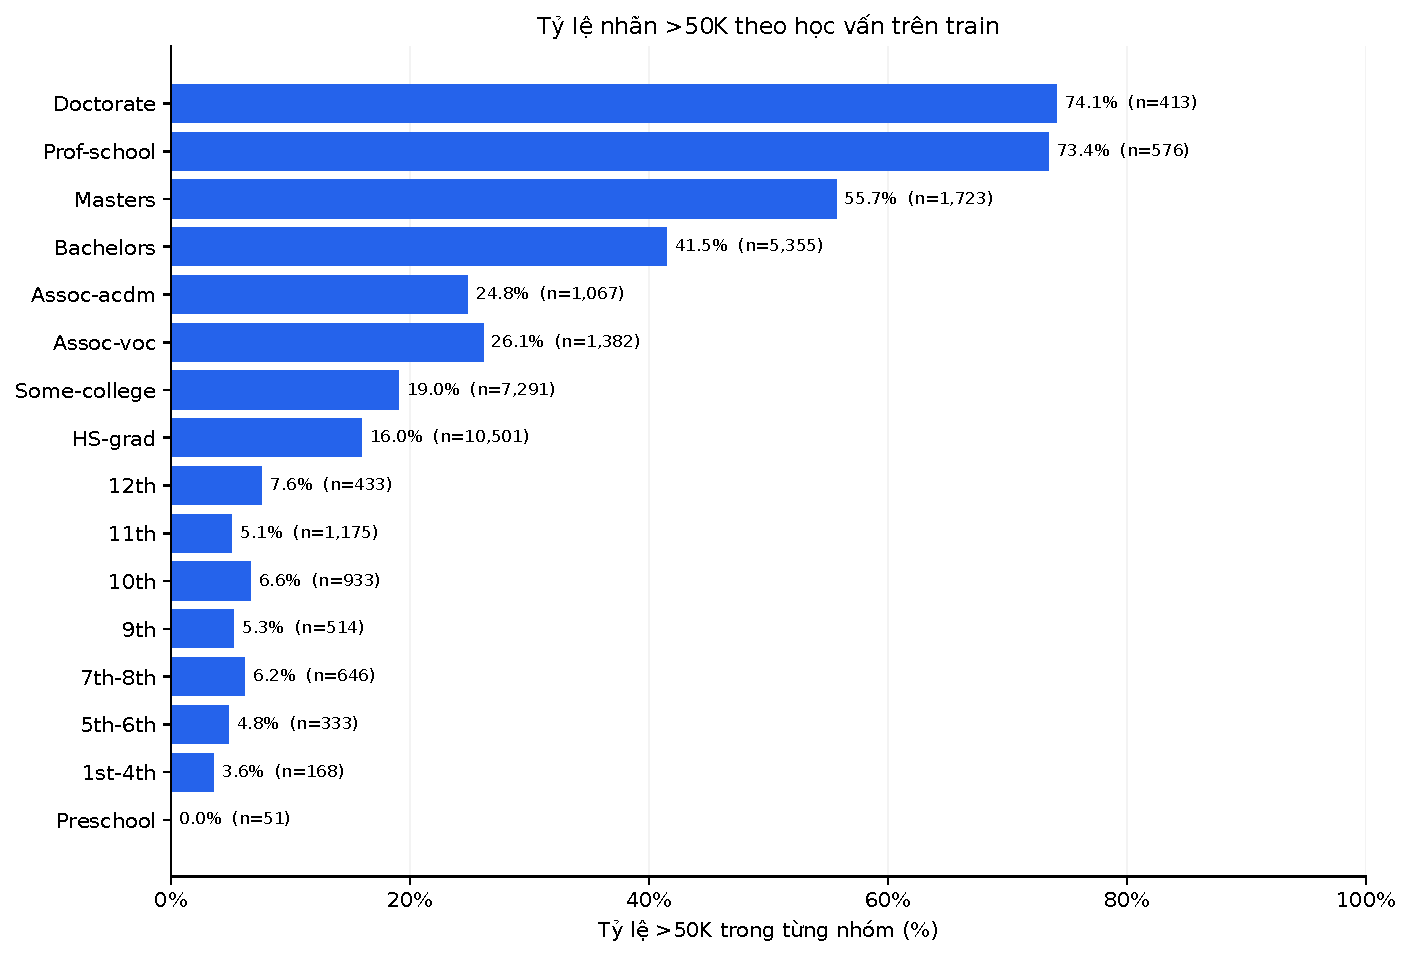
\includegraphics[width=.92\textwidth,height=.72\textheight,keepaspectratio]{Images/chapter_3/3_6/education_income_rate.pdf}
\caption{Tỷ lệ lớp thu nhập cao theo học vấn, kèm số mẫu của từng nhóm}
\label{fig:education-income-rate}
\end{figure}
